%格式控制
\documentclass{Head}
\begin{document}
\linenumbers
\tableofcontents
  \enabstract{
  \lipsum[1]
  }
\section{Introduction} % (fold)
  There is a great deal of interests in the development of viable green technologies aimed at the enhancement of biodegradable and biocompatible polymer materials, such as the blend of poly $\varepsilon$-caprolactone (PCL) and polylactide (PLA)
  Blending is a low cost, easy implement process for modification of polymer mixture.
  Mixing several immiscible polymer with different physical and chemical properties has possibility to improve the overall constituents' performance. 


  Nowadays, the blending material of poly $\varepsilon$-caprolactone (PCL) and polylactide (PLA) shows a wide application in many areas. 
  PLA has excellent biocompatibility, biodegradability and dynamic property, which shows broad prospects for tissue engineering development and other areas. 
  But pure PLA has some drawbacks, including poor toughness, low degradation rate.
  Moreover, the crystallinity of PLA is low.
  These drawbacks severely restrain the application of PLA material. 
  Researchers have attempted some polymer to make blends with PLA. 
  PHB, PCL, PP and other material which has good performance has been attempted in recent years. %此处补全引用,参考RN73


  Physical property improvement has been found in some researchers'  blending experiments. 
  PCL 
  The blend of PCL and PLA shows high degradation rate , better tensile strength, which is the properties originated from PLA, while PCL with much slower degradation rate and better toughness.
  The blend of PCL and PLA is a promising material which can meet the requirement of environment and physical conditions.
  Qiaolian Lv et al.\cite{RN73} used an injection molding blend of PCL and PLA.
  They got a maximum $\sigma=29.8\pm0.9$ MPa and $E=922.5\pm9.8$ Mpa. 
  For electrospun process, Pisani et al.\cite{RN58} got a maximum $E=49.10\pm0.12$ Mpa.


  The physical property of PCL-PLA blend depends on the super molecular structure, which is dominated by the crystallization condition.
  The melting point ($T_m$) and glass transient temperature ($T_g$) of PCL are far lower than those of PLA, and the crystallization temperature ($T_c$) of PCL is even lower than the Tg of PLA. 
  Someone's research manifests that the presence of minor PCL phase favors cold crystallization of PLA in their blend system because PCL is in its molten state during PLA crystallization, reducing system viscosity as a result, or acts as additional substrates.


  %本实验研究的目的
  The goal of this research work to improve the physical properties of the blend. 
  Stretching of the electrospun mat induces the inner fibers to align in one direction. 
  The unmolten PLA fibers offer crystallization loci for PCL phase.
  On the other hand, the molten PCL phase favors cold crystallization of PLA fibers.
  The present works lack this kind research method.
  Does this process improve the performance of blends? This question interests the author.
  Therefore, in this work electrospinning, stretching and hot pressing experiments are carried.
  Lots of morphology, microstructure, dynamic and thermal properties are characterized.
  %此处补全引用,参考RN73 intro部分原文。
\label{sec:introduction}
  
  % section introduction (end){}
\section{Experiment}
  \subsection{Sample Preparation} % (fold)
   \label{sub:sample_preparation}
   Firstly, electrospinning process was carried out.
   PLA was supplied by %此处补全厂商信息
   PCL was supplied by %此处补全厂商信息
   20 wt\% PCL solution and 20 wt\% PLA solution were prepared. 
   2 nozzles containing PCL solution and 1 nozzle containing PLA solution were used in the electrospinning process, 
   so the mass ratio of PLA : PCL was  33:67.
   The electrospinning voltage was set at 8 keV.
   The humidity of electrospun environment was 40\%, the temperature was 25 $\mathrm{^o C}$. %此处补全湿度温度等其他纺丝参数。
   The electrospun mats were made as standard size samples.


   On the next stage, the electrospun mat was stretched by a mechanical tester. 
   The electrospinning mats were stretched to a series of elongation ratios. 
   The velocity of the tensile process was 4 mm/minute, which is a low speed to avoid the fracture of the samples.
   25\%, 50\%, 75\%, 100\% and 125\% elongation ratio mats were made.
   After that the mats' double edges were fixed by heat-resistant tape in order to keep the elongation status since the mats had a rebound trend.
   Subsequently, the extended mats were put between two foils which stuck to 300 $\mathrm{^o C}$-resistant film. 
   The mats were deposited in a heat oven which kept an 80 $\mathrm{^o C}$ environment lasting 1 hour for PCL's melting.
   After 1 hour, the mats were transferred into another heat oven which kept a 30 $\mathrm{^o C}$ environment lasting 30 minutes for isothermal crystallization.


   Finally, the sample was tailored into a dimension of 10 mm $\times$ 5 mm, and the thickness was recorded by a film thickness gauge.
   Abundant standard sample with same length and width were prepared for the following characterizations.
  \subsection{Morphology and microstructure characterizations} % (fold)
  \label{sub:Morphology and microstructure characterizations}
    \subsubsection{Polarized Optical Microscope (POM)}
    POM is an effective facility to observe the microstructure of polymer material. 
    With Maltese cross phenomenon in birefringence polymer crystals, the amorphous and crystallization zone can be clearly distinguished.
    A Linkam heating stage was used to handle the electrospinning films with the same heat treatment process as the experiment in \autoref{sub:sample_preparation}. 
    The melting and the cold crystallization process of different elongation samples were observed and recorded by a Leica POM.
   
    \subsubsection{Small Angle X-ray Scattering(SAXS)}
    Small Angle X-ray Scattering(SAXS) experiment was carried on beamline BL16B1, Shanghai Synchrotron Radiation Facility. 
    A Pilatus 2M detector(1475 $\times$ 1679 pixels with a pixel size of 172 mm) was performed to collect the SAXS pattern.
    The X-ray wavelength was 0.103 nm, and the sample to detector distance was set at 2131 mm. %补全19U2线站的测试条件
    Considering the scale of X-ray pattern on BL19U2 is much larger than the diameter of PLA fibers inside the samples. 
    It was essential to focus the X-ray pattern.
    A beryllium compound reflective lens(CRL) was deployed to get a 5$\mu m$ diameter X-ray pattern. 
    Besides a portable POM was placed on the light path in order to determine location on blends characterized by the SAXS method.%此处可能加图。
    %此处补全型号以及测试条件,以及考虑微聚焦偏光显微系统是否要详细介绍。


    \subsubsection{Wide Angle X-ray Scattering(WAXS)}
    WAXS experiment was carried on beamline BL16B1, Shanghai Synchrotron Radiation Facility, Pilatus 2M detector
    (1475$\times$1679 pixels with a pixel size of 172 mm). The X-ray wavelength was 0.124 nm, and the sample to detector distance was set at 178.5 mm.
  \subsection{Dynamic Property Characterization} % (fold)b'b
  \label{sub:dynamic_property_characterization}
  The dynamic properties of the neat PCL and its blends with various annealing histories were determined by a mechanical tester at a crosshead speed of 50 $\mathrm{mm\cdot min^{-1}}$) at 25 $\mathrm{^o C}$ using the dog-bone shaped specimens.
  Strength and modulus values reported here represent an average of the results for tests run on 6 specimens.


  \subsection{Thermal Property Characterization} % (fold)
  \label{sub:thermal_property_characterization}
    \subsubsection{Thermogravimetric Analysis (TGA)}
    TGA measurements were carried out in a Mettler Toledo TGA 2 thermal analyzer. 
    The experiments were performed under nitrogen atmosphere(flow rate of 50 $\mathrm{mL\cdot min^{-1}}$). 
    Each sample was heated from 0 $\mathrm{^o C}$ to 600 $\mathrm{^o C}$ at 10 $\mathrm{^o C\cdot min^{-1}}$.
    The initial degradation temperatures ($T_0$) were determined at 5\% mass loss, whereas temperatures at the maximum degradation rate ($Tmax$) were calculated from the first derivative of the TGA curves (DTG).


    \subsubsection{Differential Scanning Calorimetry (DSC)}
    DSC's experiments were performed in a Mettler Toledo DSC 3+ under nitrogen atmosphere (flow rate of 50 $\mathrm{mL\cdot min^{-1}}$). 
    Sample weights of 2 mg were sealed in aluminum pans and heated from 0 $\mathrm{^o C}$ to 200 $\mathrm{^o C}$ at 10 $\mathrm{^o C\cdot min^{-1}}$. 
    The degree of crystallinity($\chi_{c}$) was calculated through \autoref{eq1}
    
    \begin{equation}
      \chi_{c}=100\%\times[{}\frac{\Delta H_m -\Delta_{cc}}{\Delta H^c_m }]\frac{1}{W_{PCL}}
      \label{eq1}
    \end{equation}
  % subsection saxs_ch (end)
  
  % subsection thermal_property_characterization (end)
  
  % subsection dynamic_property_characterization (end)
  
  % subsection polarize_optical_observation (end)
   
   % subsection mat_preparation (end) % (fold)
  \label{sec:experiment}
  \section{Result and Analysis} % (fold)
  As shown in,a is the melting and isothermal crystallization of 0 \% elongation sample, b is
  the same process of 125 \% elongation sample. Compare the evolution of two samples, it can be
  remarkably noticed that the stretching force make PLA fibers inside samples  present a certain degree of orientation.
  During the isothermal crystallization process at 30 $\mathrm{^o C}$ , the PCL grain firstly appears on the surface of
  PLA fiber. After a short time, the grain is fill the entire matrix.
    \subsection{Crystallization behavior}
    \begin{figure} %图片浮动体
      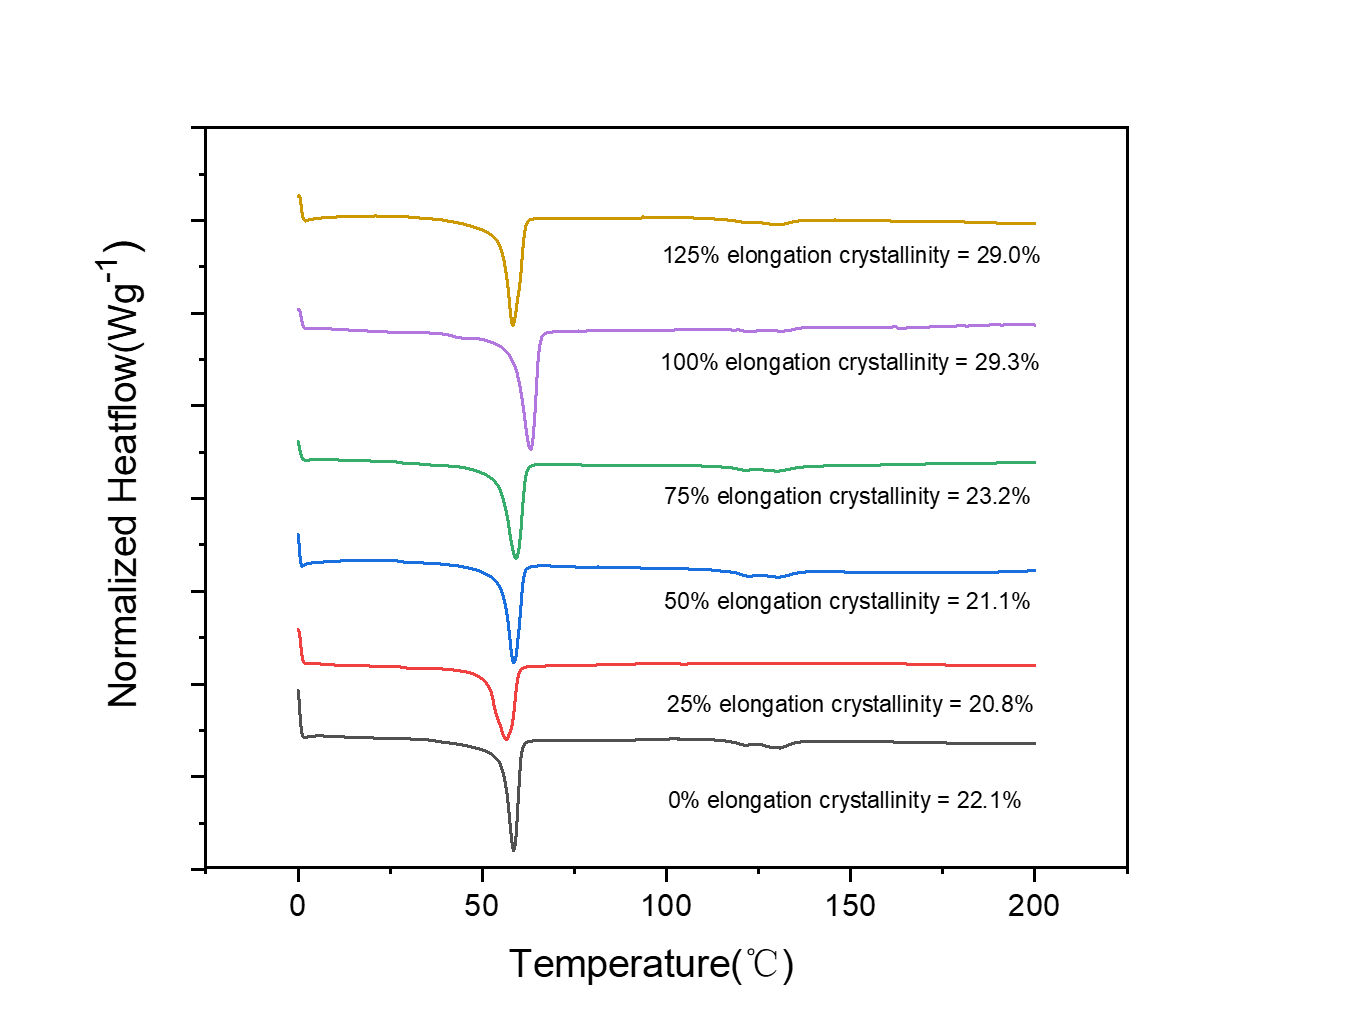
\includegraphics[scale = 0.5]{figures/DSC_result_1.png}
    \end{figure}
    \label{sec:result_and_Analysis}
    \renewcommand{\tablename}{\textbf{Table}}
    \captionsetup[table]{labelsep = period}
    \begin{table} %表格浮动体
      \caption{Crystallinity of components in PCL/PLA blends}
      \begin{tabular}{cccc}
      \toprule
      Sample & Crystallinity (\%) of PCL phase & Crystallinity (\%) of PLA phase & Melting point($\mathrm{^o C}$) of PCL phase\\
      \midrule
      0\% & 22.1 & - & 58.7\\
      25\% & 20.8 & - & 56.6\\
      50\% & 21.1 & - & 58.6\\
      75\% & 23.2 & - & 59.1\\
      100\% & 29.3 & - & 63.0 \\
      125\% & 29.0 & - & 58.5 \\
      \bottomrule
      \label{DSC_result_table}
      \end{tabular}
      $\chi_c $ calculated using $\Delta_m^c$ of PCL of 139.5($\mathrm{J\cdot g^{-1}}$)
    \end{table}
  \section{Conclusion} % (fold)
  \label{sec:conclusion}
  
  % section conclusion (end)
  % section result_and_analysis (end)
  % section experiment (end)
  \section{Acknowledgement} % (fold)
  \label{sec:acknowledgement}
  
  % section acknowlagement (end)
  \bibliography{ref}
  \end{document}